\chapter{Data and Preprocessing}
\label{ch:data}

The work uses a corpus of twenty-one active-region magnetic
winding-flux cubes derived from vector magnetograms recorded by the
Helioseismic and Magnetic Imager (HMI)~\cite{scherrer2012hmi} aboard
the Solar Dynamics Observatory (SDO)~\cite{pesnell2012sdo}. Each
cube is computed from the HMI Space-weather HMI Active Region Patch
(SHARP) vector-magnetogram products~\cite{bobra2014sharp,hoeksema2014hmi}
by integrating the winding-flux density of Prior \& MacTaggart along
the line-of-sight component of the photospheric field, and is stored
as a Zarr archive at 12-minute cadence. This chapter documents the
on-disk format, the locked physical priors, the chiral augmentation
rule, the splits, the winding-flux outlier guard, and the bucketed
sampler used to incorporate cubes of variable spatial extent within
a single training run.

\section{On-disk format}
\label{sec:data-format}

Each cube is a Zarr group containing two arrays: a single-channel
field $\mathtt{wind}\,[H,W,T]$ of \texttt{float32} winding-flux
values, and a one-dimensional \texttt{float64} array
$\mathtt{Time}\,[T]$ of Unix-epoch seconds. The axis convention is
locked as $[H,W,T]$ with $W$ mapped to the heliographic $X$ axis and
$H$ to the heliographic $Y$ axis. No coordinate arrays and no
\texttt{.zattrs} payload are present; the only metadata available
is the HMI Active Region Patch (HARP) identifier encoded in the
directory name. This minimal format is treated as final for the
scope of this work; no additional metadata or coordinate arrays are
assumed to be available.

\begin{figure}[htbp]
\centering
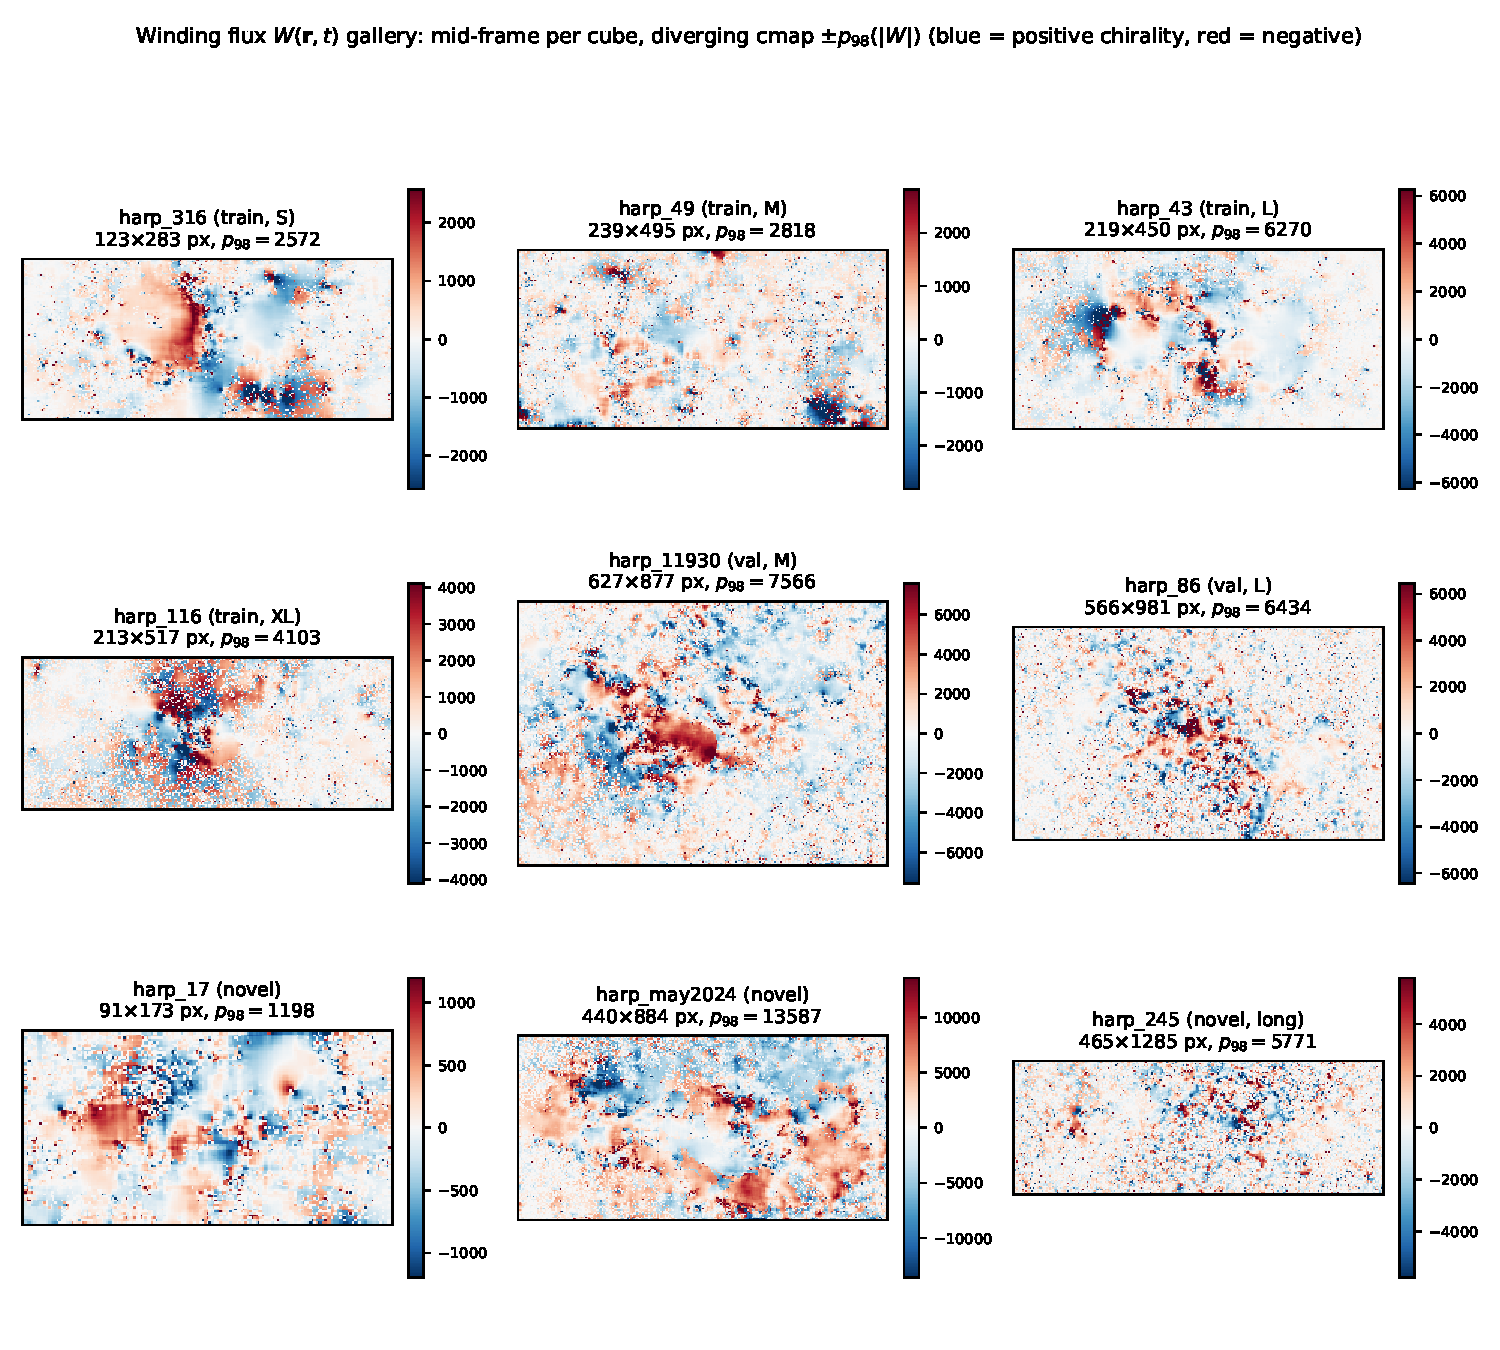
\includegraphics[width=\linewidth]{assets/figures/wind_gallery.pdf}
\caption{Gallery of representative winding-flux frames sampled
across the corpus. Each panel shows the mid-frame of one cube on
a diverging colourmap with symmetric range $\pm p_{98}(|W|)$
(blue $\equiv$ positive chirality, red $\equiv$ negative); the
panel title records the cube identity, split membership, and the
pixel-area bin. The variable spatial extent that motivates the
bucketed sampler of \S\ref{sec:data-sampler} is visible directly,
as is the bipolar lobe structure (paired blue and red regions)
that is the load-bearing chiral signal the encoder is asked to
learn.}
\label{fig:wind-gallery}
\end{figure}

\begin{figure}[htbp]
\centering
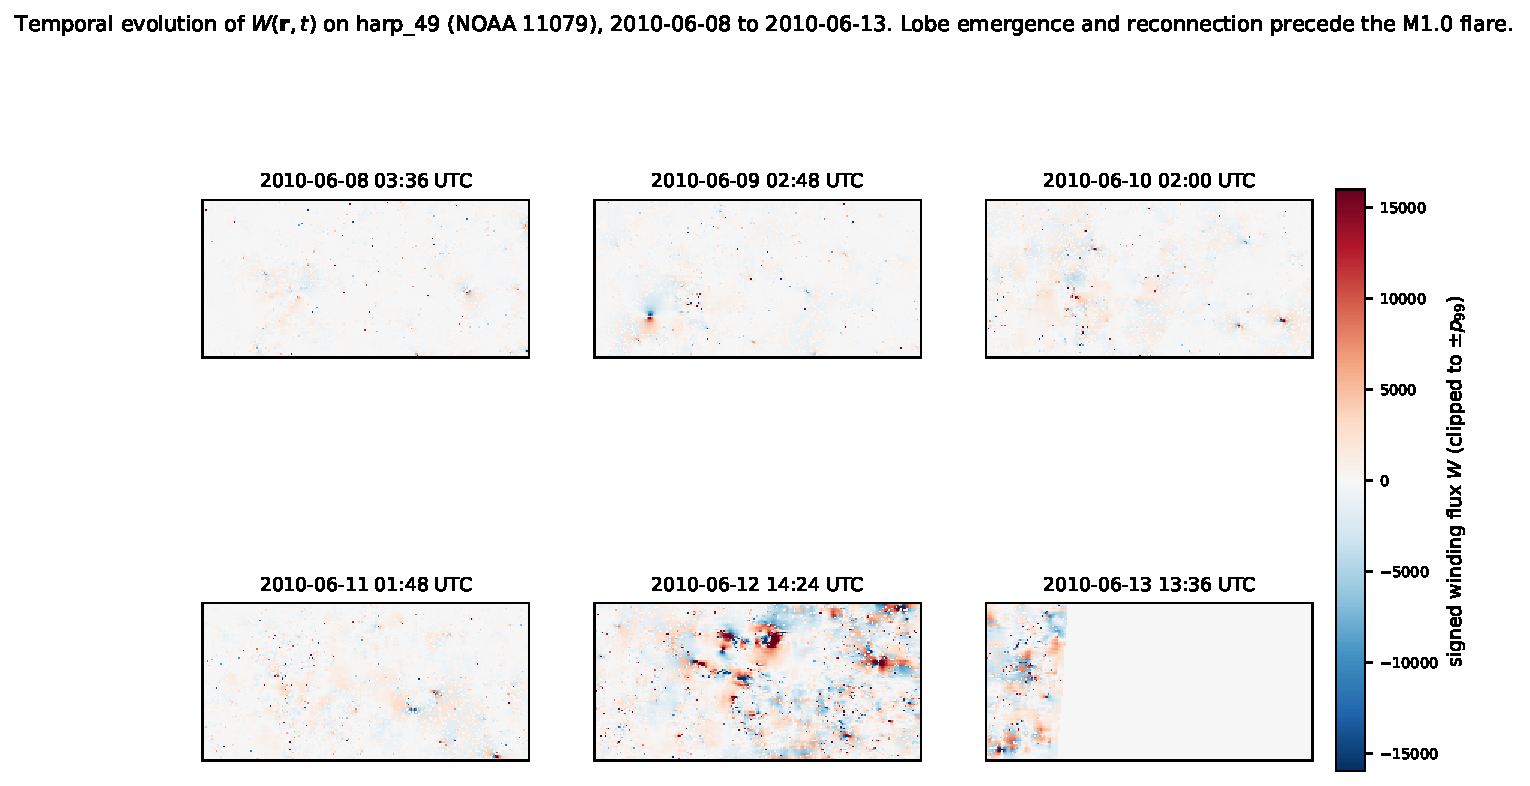
\includegraphics[width=0.98\linewidth]{assets/figures/wind_time_evolution.pdf}
\caption{Temporal evolution of $W(\mathbf{r},t)$ on harp\_49
(NOAA~11079) sampled at six near-equispaced UTC time stamps over
the 2010-06-08 to 2010-06-13 observation window, on a common
diverging colourmap with symmetric range $\pm p_{99}(|W|)$. The
active region is photometrically quiescent on the first three
days, develops a dominant bipolar lobe by 2010-06-09, undergoes
a structured re-organisation through 2010-06-11 and 2010-06-12,
and produces the spike pattern reported in
Figure~\ref{fig:precursor-demo} on 2010-06-12 prior to the
catalogued M1.0 flare on 2010-06-13. The spatial non-stationarity
demonstrated here is the structure on which the JEPA encoder
must learn to predict in embedding space.}
\label{fig:wind-time-evolution}
\end{figure}
\FloatBarrier

\section{Locked physical priors}
\label{sec:data-priors}

The following priors are locked for the entire project and are
relied upon throughout the architecture (Chapter~\ref{ch:architecture}):
\begin{itemize}\setlength\itemsep{0pt}
\item pixel scale $0.364\,\mathrm{Mm/px}$, constant across cubes,
inherited from the HMI plate scale of $0.5^{\prime\prime}/\mathrm{px}$
at $1\,\mathrm{AU}$~\cite{scherrer2012hmi};
\item cadence $720\,\mathrm{s}$ (12 minutes), enforced by the loader as
$|\,\mathrm{median}(\Delta t)-720\,| < 1\,\mathrm{s}$;
\item the field is a signed chiral pseudoscalar, not a magnetic-field
strength;
\item per-pixel physical maximum $|w|_{\max} \approx 10^{7}$ in
the native units of the winding-flux density of
Prior~\&~MacTaggart (Gauss times megametre squared in the
source-pipeline convention; carried as a dimensionless raw float
throughout the model since the encoder is normalisation-invariant);
\item integrated active-region totals fall in the
$10^{13}$--$10^{14}$ range.
\end{itemize}

\section{Sparse-storage and time semantics}
\label{sec:data-sparse}

The Zarr chunks omit blocks whose values are entirely zero; reads
silently materialise such blocks as zeros, with the consequence that
a zero pixel may correspond to one of three classes (sparse fill,
off-AR padding, or a genuine near-zero winding flux). These three
classes are numerically indistinguishable at the model input and are
treated as a single \emph{numerically valid} class. A fourth class
--- pixels flagged as instrument-invalid or off-disk --- is encoded as
\texttt{NaN} on disk and is propagated as a separate boolean
\emph{valid-pixel mask} that enters the loss-mask intersection
of equation~\eqref{eq:lossmask}.

The $\mathtt{Time}$ array uses the sentinel value $0$ for unfilled
slots; the loader filters to $\mathtt{Time}>0$ before sampling any
window, so that no window straddles an unfilled slot. The cadence
assertion above then verifies that the surviving frames are
uniformly spaced at $720\,\mathrm{s}$.

\section{Winding-flux outlier guard}
\label{sec:data-clip}

A small number of pixels in the corpus carry values that exceed the
physical maximum by several orders of magnitude. An earlier version
of the loader applied a guard of $10^{5}$ on the assumption that the
quantity was a magnetic-field strength expressed in Gauss; this
guard was found to destroy legitimate signal in the $10^{5}$--$10^{7}$
range. The current guard is set at $|w| > 10^{8}$, a tenfold safety
margin above the physical maximum, and is implemented in
\texttt{solarflare\_data/zarr\_loader.py}. Pixels that exceed the
guard are zeroed in the input and excluded from the loss via the
valid-pixel mask. Table~\ref{tab:clip-audit} summarises the
twenty-one-cube outlier audit; the full audit is reproduced in
Appendix~\ref{app:clipping}.

\begin{table}[htbp]
\centering\small
\begin{tabular}{l r r r r}
\toprule
Cube & $T$ & $n_{>10^{8}}$ & frac & peak $|w|$ \\
\midrule
\textbf{harp\_8}  &  732 & \textbf{14{,}220} & $1.5\times10^{-4}$ & $1.68\times10^{10}$ \\
harp\_11930        &  325 & 832 & $5\times10^{-6}$ & $1.99\times10^{8}$ \\
harp\_54           &  445 & 302 & $4\times10^{-6}$ & $2.44\times10^{8}$ \\
harp\_43           &  927 & 246 & $3\times10^{-6}$ & $1.27\times10^{8}$ \\
harp\_49           &  651 &  86 & $1\times10^{-6}$ & $4.56\times10^{8}$ \\
ten further cubes  &  --- & $\leq 191$ & $\leq 2\times10^{-6}$ & $\leq 6.15\times10^{7}$ \\
\bottomrule
\end{tabular}
\caption{Pathological pixel counts above the $10^{8}$ guard.
\texttt{harp\_8} carries thirty times the per-cube outlier count of
its nearest neighbour and is the only cube whose standard deviation
collapses by more than a factor of twenty under the guard
($3.8\times10^{6} \to 1.7\times10^{5}$).}
\label{tab:clip-audit}
\end{table}

\section{Chiral augmentation}
\label{sec:data-aug}

Because the winding-flux density $w$ is a chiral pseudoscalar
under spatial inversion~\cite{prior2020helicity},
transforms that change the handedness of the spatial frame must be
paired with an explicit sign flip. Table~\ref{tab:d4} enumerates the
augmentation set, which forms the dihedral group $D_{4}$ acting with
chirality. Time
reversal and random cropping are disabled: time reversal converts
forecasting into hindcasting (physically wrong); random cropping
discards spatial extent that the variable-shape sampler is already
exploiting.

\begin{table}[htbp]
\centering\small
\begin{tabular}{l c l}
\toprule
Transform & Sign action & Augmented sample \\
\midrule
Identity                 & $+$ & $x'\;=\;x$ \\
Horizontal flip          & $-$ & $x'\;=\;-\mathrm{flip}_{H}(x)$ \\
Vertical flip            & $-$ & $x'\;=\;-\mathrm{flip}_{V}(x)$ \\
$90^{\circ}$ rotation    & $-$ & $x'\;=\;-\mathrm{rot}_{90}(x)$ \\
$180^{\circ}$ rotation   & $+$ & $x'\;=\;\mathrm{rot}_{180}(x)$ \\
$270^{\circ}$ rotation   & $-$ & $x'\;=\;-\mathrm{rot}_{270}(x)$ \\
\bottomrule
\end{tabular}
\caption{Chirality-aware $D_{4}$ augmentation: each row applies a
spatial transform and the indicated sign correction.}
\label{tab:d4}
\end{table}

\section{Splits}
\label{sec:data-splits}

The splits are constructed at the cube (HARP-identity) level to
eliminate active-region leakage between train, validation, and
holdout. The thesis run~E30 uses thirteen cubes for training, three
for validation, and reserves five cubes as a strict holdout for the
downstream probe of Chapter~\ref{ch:probe}. The full assignment is
recorded in Table~\ref{tab:splits}.

\begin{table}[htbp]
\centering\small
\begin{tabular}{l p{0.65\linewidth}}
\toprule
Partition & HARP identities \\
\midrule
Train (13)    & harp\_8, harp\_26, harp\_43, harp\_45, harp\_49,
                harp\_54, harp\_83, harp\_116, harp\_156, harp\_219,
                harp\_274, harp\_316, harp\_318 \\
Val (3)       & harp\_86, harp\_221, harp\_11930 \\
Novel (5)     & harp\_17, harp\_51, harp\_245, harp\_may2024,
                harp\_nov2025 \\
\bottomrule
\end{tabular}
\caption{Cube-level partitioning for the E30 thesis run. The split
is constructed by stratifying the twenty-one cubes into four
spatial-extent bins (S, M, L, XL by pixel area) and assigning by
the rule of \S\ref{sec:data-splits}. The novel five are unseen by
the encoder at all stages.}
\label{tab:splits}
\end{table}

The five holdout cubes are selected to span the operating regimes
of the downstream probe rather than uniformly at random.
Specifically: harp\_17 and harp\_51 are the active regions used as
wind-probe anchors during the earlier E09/E11 sanity-scale
investigation, retained as cross-checkpoint comparison points;
harp\_may2024 and harp\_nov2025 are the two most-recent active
regions in the corpus, supplying a temporal-domain-shift test;
and harp\_245 is the longest cube in the corpus at 1\,472 frames
and the heavy-tailed target distribution that motivated the
log-affine calibration of \S\ref{sec:probe-logcal}. The training
partition retains all four XL-bin (above $400\,\mathrm{k}$
pixels) cubes so that the encoder sees the maximum-resolution
diversity available, and the cube harp\_8 is retained in training
for its clip-edge outlier signal (\S\ref{sec:data-clip}). Smaller
experiments (Chapter~\ref{ch:experiments}) use the same
partitioning rule on a reduced cube count.

\section{Bucketed variable-shape sampler}
\label{sec:data-sampler}

Cubes vary in spatial extent from $(376\times376)$ to
$(877\times1061)$ pixels. A bucketed sampler groups cubes of
similar $(H,W)$ and draws fixed-shape windows of $T = t_{\text{in}}
+ t_{\text{out}} = 14$ contiguous frames from within a bucket per
mini-batch. Gradient accumulation across buckets is used to
construct a single optimiser step from heterogeneous batches. Each
window is required to contain only $\mathtt{Time}>0$ entries; windows
that fail this test are rejected and re-drawn.

\begin{figure}[htbp]
\centering
\begin{tikzpicture}[
  >=stealth, font=\small,
  node distance=0.55cm and 0.7cm,
  stage/.style={draw, rounded corners, align=center, minimum width=2.6cm,
                minimum height=0.95cm, fill=blue!8},
  store/.style={draw, cylinder, shape border rotate=90, aspect=0.25,
                align=center, minimum height=1.0cm, minimum width=1.8cm,
                fill=gray!10},
  slabel/.style={align=center, font=\scriptsize\ttfamily},
  arr/.style={->, thick}]

  \node[store] (zarr) {\texttt{harp\_*.zarr}\\\scriptsize{wind\,$[H,W,T]$}};
  \node[stage, right=of zarr] (samp) {bucketed sampler\\\scriptsize{group by $(H,W)$}};
  \node[stage, right=of samp] (pad) {reflect-pad\\\scriptsize{to multiple of $P=16$}};
  \node[stage, below=1.2cm of pad] (lift) {$1\!\times\!1$ conv\\\scriptsize{$1\!\to\!13$ channels}};
  \node[stage, left=of lift] (patch) {ViT patchify\\\scriptsize{$P=16,\,t=2$}};
  \node[stage, left=of patch] (tok) {token sequence\\\scriptsize{$[B,\,T h_p w_p,\,d{=}384]$}};

  \node[slabel, above=0.05cm of zarr] {$H{\times}W{\times}T$};
  \node[slabel, above=0.05cm of samp] {$[B,T,1,H,W]$};
  \node[slabel, above=0.05cm of pad]  {$[B,T,1,H_p,W_p]$};
  \node[slabel, above=0.05cm of lift] {$[B,T,13,H_p,W_p]$};
  \node[slabel, above=0.05cm of patch]{$[B,T,13,h_p,w_p]$};
  \node[slabel, above=0.05cm of tok]  {$[B,N,d]$};

  \draw[arr] (zarr) -- (samp);
  \draw[arr] (samp) -- (pad);
  \draw[arr] (pad)  -- (lift);
  \draw[arr] (lift) -- (patch);
  \draw[arr] (patch) -- (tok);

  \node[draw, dotted, rounded corners, fit=(pad)(lift)(patch),
        inner sep=0.25cm, label={above:\scriptsize input adapter (\S\ref{sec:arch-adapter})}] {};
\end{tikzpicture}
\caption{Data pipeline from on-disk Zarr cube to ViT token
sequence. Tensor shapes annotated above each stage:
$(H,W)$ is per-cube; $(H_p, W_p)$ is the reflection-padded
size to the next multiple of patch size $P{=}16$; $h_p=H_p/P$
and $w_p=W_p/P$ are the spatial-token-grid dimensions; $T$ is
the window length and $N = T h_p w_p$ the per-window token
count. The boolean $M_{\text{pad}} \in \{0,1\}^{h_p \times w_p}$
mask is propagated alongside the embedded tensor (not drawn)
and intersected with the loss mask so padded positions never
enter the gradient.}
\label{fig:data-pipeline}
\end{figure}
\FloatBarrier
